    %\begin{frame}{Описание разработанного метода}
    %    Данный метод подходит не только для английского, он подходит для любого языка семантикa которого, будет описанa на языке Universal Dependencies.
    %\end{frame}
    %\begin{frame}{Результаты семестра}
    %    \begin{itemize}
    %        \item Выбрано вспомогательное средство разработки, а именно парсер английского языка, разработанный Стенфордским университетом.
    %        \item На основе документации парсера, а так же описание формата его вывода, написан алгоритм выделения перечислений.
    %    \end{itemize}
    %\end{frame}
    %\begin{frame}{Обоснование тестирования}
    %    С парсером в комплекте идет порядка 15 тысяч тестов. Из них мы выделили строки содержащие союзы,
    %    а так же знаки пунктуации указывающие на возможные перечисления. Список сократился до 9600 тестов.\\
    %    На данный момент я нахожусь в процессе занесения тестов в базу.\\
    %    После внесения тестов в базу, следующим шагом будет анализ полноты этой базы, и добавление недостающих тестов.
    %\end{frame}
    %\begin{frame}{Метод}
    %\huge    \textbf{Предположим нам дано предложение:} \\
    %    John and Peter go to the cinema as well as to the park. \\
    %    Определим перечисления данного предложения.\\
    %\end{frame}
    %\begin{frame}{Метод}
    %  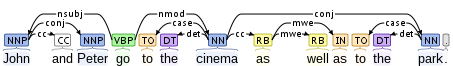
\includegraphics[width=\textwidth]{./example.png} \\
    %  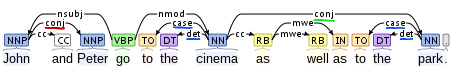
\includegraphics[width=\textwidth]{./example2.png} \\
    %  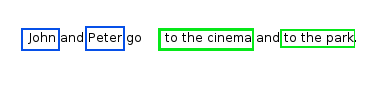
\includegraphics[width=\textwidth]{./example_result.png} 
    %\end{frame}
    %\begin{frame}{Метод}
    %    \textbf{Используемые связи:}
    %    \begin{enumerate}
    %        \item \textbf{appos} - связь соединяющая определение для модификации существительного, если идет сразу после существительного, примеры и
    %        сокращения, (при наличии нескольких, конкурирующих; пары ключ-значение(адрес , телефон и прочее)) с существительным
    %        \item \textbf{list} - связь используется для цепочек состоящих из более чем двух элементов. так же для последовательностей атрибутов, или
    %        \item описательных терминов(веб тексты)
    %        \item \textbf{conj} - связь элементов соединенных элементом-соединителем(cc или punct), связь начинается с первого элемента и идет к
    %        остальным
    %        \item \textbf{remnant} - связь при использовании повторения похожих простых предложений в сложном если во втором и последующих опущен
    %        глагол (Marie went to Paris and Miriam to Prague)\\
%            \item Связь типа List, второй и последующие элементы можно менять местами(лексемы внутри элементов связаны appos).
%            \item Связь типа Remnant второй и последующие элементы можно менять местами.
%            \item Связь типа Appos второй и последующие элементы можно менять местами.
%            \item Связь типа Conj элементы можно менять местами.
    %    \end{enumerate}
    %\end{frame}
    %\begin{frame}{Перечисление}
    %    \Large \textbf{Перечисление} - последовательность элементов в ответе, элементы которой могут быть переставлены не порождая ошибки. \\
    %    Элементы перечисления могут быть разделены лексемами-разделителями.\\
    %    Элементы перечисления не могут иметь общих лексем.\\
    %    Перечисления могут быть вложены, т.е. одно может быть элементом другого.
    %    В естественных языках это однородные члены, а также части сложносочиненного предложения.
    %\end{frame}
    %\begin{frame}{AS-IS}
    %  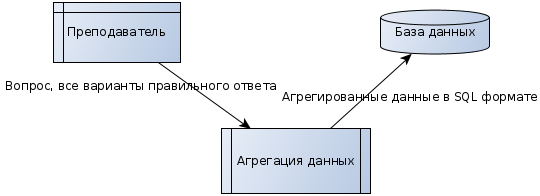
\includegraphics[width=\textwidth]{./dfd_create_as_is.png}
    %\end{frame}
    %\begin{frame}{TO-BE}
    %  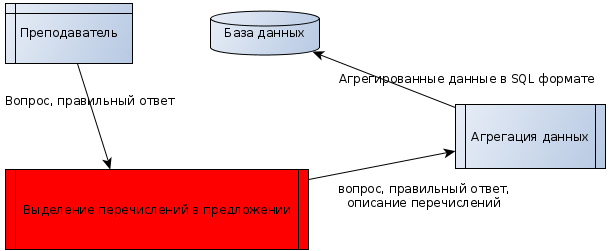
\includegraphics[width=\textwidth]{./dfd_create_to_be.png}
    %\end{frame}
    %\begin{frame}{AS-IS}
    %  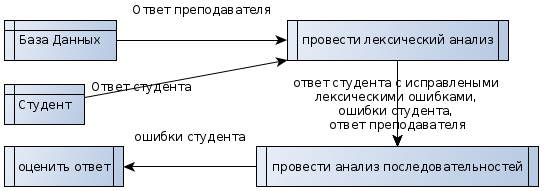
\includegraphics[width=\textwidth]{./dfd_measure_as_is.png}
    %\end{frame}
    %\begin{frame}{TO-BE}
    %  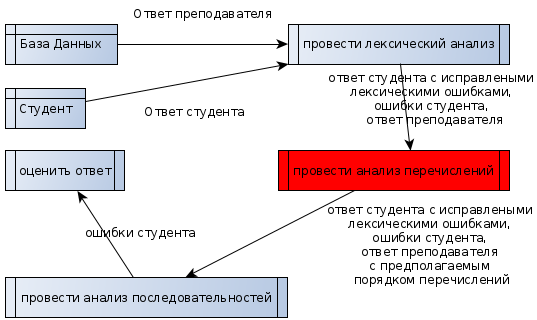
\includegraphics[width=\textwidth]{./dfd_measure_to_be.png}
    %\end{frame}
%\begin{frame}{Постановка задачи}
%    \small\textbf{Дано:} T = <A,S> \\
%    \small 
%    \hspace{0.5cm}\textbf{T} - Пара ответов для проверки \\
%    \hspace{0.5cm}\textbf{A} - Эталонный ответ с описаниями лексем\\
%    \hspace{0.5cm}\textbf{S} - Ответ студента \\
%     Ответы являются упорядоченными множествами лексем. \\
%    \hspace{0.5cm}\textbf{Q} - Множество эталонных ответов с описаниями лексем. \(\forall A \in Q\)\\
%    \textbf{Цель:} минимизировать |Q|, при сохранении корректности Q. \\
%    \textbf{Решение:} 
%    Модифицировать ответ: T = <A,S,E> \\
%Разработать функцию: F(A,S,E) \\
%    \small \hspace{0.5cm}\textbf{E} - Множество описаний перечислений в эталонном ответе\\
%    \small \hspace{0.5cm}\textbf{F} - Функция генерации множества эталонных ответов на основе описания перечислений и ответа студента. \\
% \(\forall e \in E, e = \{z | \exists x \exists y (z = (x,y)) \}\), \\
%     \(\forall z \in e, \forall e \in E, x \leq y, \forall x \leq n, \forall y \leq n \) \\
%    \small \hspace{0.5cm}\textbf{z} - Описание элемента перечисления \\
%    \hspace{0.5cm}\textbf{x,y} - Индексы первой и последней лексем элемента перечисления, в эталонном ответе \\ 
%    \hspace{0.5cm}\textbf{n} - Количество лексем в эталонном ответе  \\ 
%    \( x_1,y_1 \in z_1, x,y \in z, \forall z \in e, \forall e \in E, \forall z_1 \in e_1, \forall e_1 \in E, \nexists z \nexists z_1 ([x <  x_1 < y \land x_1 < y < y_1] \lor 
%[x_1 < x < y_1 \land x < y_1 < y]) ) \) \\
%\end{frame}
    %\begin{frame}{Фиксация проблемы}
    %    Отсутствие автоматизации обработки перечислений для английского языка в тестовых вопросах систем дистанционного обучения.
    %\end{frame}
    %\begin{frame}{Диагностика проблемы}
    %    \begin{itemize}
    %        \item Проблемой является трудоемкость создания вопроса, который содержит перечисления(однородные члены), так как необходимо перебрать все порядки элементов для каждого перечисления.
    %        \item Наличие перечислений и необходимость ввода множества вариантов правильного ответа, влечет за собой проблему создания ошибочного вопроса из-за человеческого фактора. \\
    %        \item Учитывая сложность создания вопросов с однородными членами, часть учителей откажутся от использования однородных членов, что приведет к снижению качества тестов и их ограниченности.\\
    %    \end{itemize}
    %\end{frame}
    %\begin{frame}{Список стейкхолдеров}
    %    \begin{itemize}
    %        \item Учителя связанные с разработкой курсов для СДО
    %        \item Организации использующие электронные курсы обучения английскому
    %        \item Ученики изучающие английский с помощью СДО
    %        \item Будущие поколения
    %        \item Государства, один из официальных языков, которых английский
    %    \end{itemize}
    %\end{frame}
    %\begin{frame}{Выявление "проблемного месива"}
    %    \begin{enumerate}
    %        \item Сложность создания вопросов с однородными членами;
    %        \item Сложность и трудоемкость проверки ответов с однородными членами;
    %        \item Сложность написания ответа для студента( студент может быть запутаться в большом количестве вариантов ответа,
    %                          не зная равноценны ли они);
    %        \item Низкий уровень знаний английского из-за ограниченности курсов дистанционного обучения;
    %        \item Отсутствие дистанционных систем обучения поддерживающих перечисления
    %    \end{enumerate}
    %\end{frame}
    %\begin{frame}{Дерево проблем}
    %  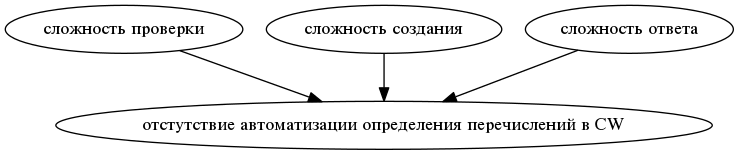
\includegraphics[width=\textwidth]{./problem-tree.png}
    %\end{frame}
    %\begin{frame}{Дерево целей}
    %  
\includegraphics[width=\textwidth]{./goal-tree.png}
    %\end{frame}

    %\begin{frame}{Интеллектуальная карта}
    %  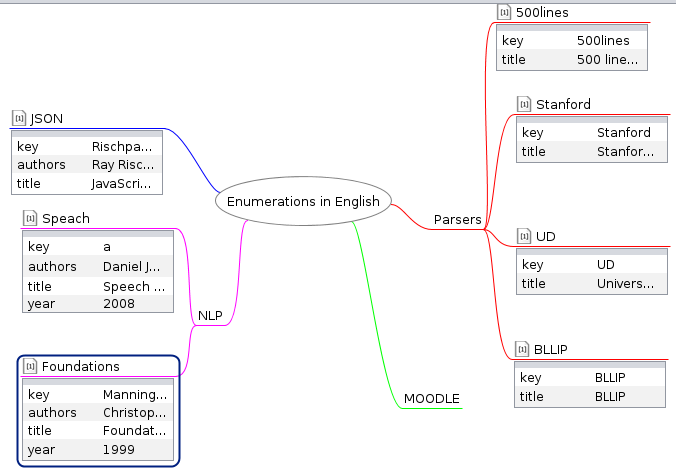
\includegraphics[width=\textwidth]{./mind_map.png}
    %\end{frame}
    %\begin{frame}{Список источников}
    %    \begin{itemize}
    %        \item Документация по BLLIP(http://bllip.cs.brown.edu/)
    %        \item Документация по парсеру в 500 строк(https://spacy.io/blog/parsing-english-in-python)
    %        \item Документация по парсеру Стенфорда(http://nlp.stanford.edu/software/lex-parser.shtml)
    %        \item Документация по языку используемому в Стенфордском парсере(http://universaldependencies.github.io/docs/)
    %        \item Daniel Jurafsky and James H. Martin. 2008. Speech and Language Processing: 
    %            An Introduction to Natural Language Processing, Speech Recognition, and Computational Linguistics. 2nd edition. Prentice-Hall.
    %        \item Christopher D. Manning and Hinrich Schütze. 1999. Foundations of Statistical Natural Language Processing. Cambridge, MA: MIT Press.
    %        \item Ray Rischpater Packt Publishing. 2015. JavaScript JSON Cookbook.
    %    \end{itemize}
    %\end{frame}
    %\begin{frame}{Объект, предмет исследования, используемые методы}
    %    \huge
    %    \textbf{Объект} - перечисления\\
    %    \textbf{Предмет исследования} - перечисления в английском языка и способы их определения\\
    %    \textbf{Используемые методы} - методы обработки естественного языка, а также методы программной инженерии
    %\end{frame}
    %\begin{frame}{Научная новизна, предполагаемая практическая ценность}
    %    \Large
    %    \begin{itemize}
    %        \item Научная новизна данной работы заключается в использовании метода на основе синтаксического анализа для определения перечислений.
    %        \item Практическая ценность состоит в расширении возможностей обучения английскому языку, за счет возможности тестирования предложений с однородными членами.
    %    \end{itemize}
    %\end{frame}
    %\begin{frame}{Актуальность}
        %\Large
        %На данный момент плагин CorrectWriting обрабатывает ответы на английском языке содержащие перечисления только при условии ввода всех вариантов правильных ответов.\\
        %Что приводит к возможности возникновения ошибок из-за человеческого фактора.\\
        %Так же необходимость ввода множества вариантов правильного ответа накладывает ограничения на использование плагина.
    %    Например в данном предложении три обстоятельства места: \\
    %    То get to her country cottage you have to ride by \textbf{the forest} , \textbf{the field} and \textbf{the lake} . \\
    %    Порождают 6 правильных вариантов ответа:
    %    \begin{enumerate}
    %        \item То get to her country cottage you have to ride by \textbf{the forest} , \textbf{the field} and \textbf{the lake} .
    %        \item То get to her country cottage you have to ride by \textbf{the forest} , \textbf{the lake} and \textbf{the field} .
    %        \item То get to her country cottage you have to ride by \textbf{the field} , \textbf{the forest} and \textbf{the lake} .
    %        \item То get to her country cottage you have to ride by \textbf{the field} , \textbf{the lake} and \textbf{the forest} .
    %        \item То get to her country cottage you have to ride by \textbf{the lake} , \textbf{the forest} and \textbf{the field} .
    %        \item То get to her country cottage you have to ride by \textbf{the lake} , \textbf{the field} and \textbf{the forest} .
    %    \end{enumerate}
        % Количество правильных ответов определяется произведением числ перестановок каждого перечислений, т.е. произведением факториалов количеств элементов каждого перечисления.
    %\end{frame}
